%!TEX root = ../main.tex

\chapter{GraphDB}
\chapterauthor{Thore Krüss, Lennart Purucker, Johanna Sommer}
\section{Abstract}
This chapter of the book gives an overview of Graph Databases as part of the NoSQL landscape, focusing on Neo4j as a specific implementation. The goal of this work is to give a timely overview of Graph Databases today as well as assessing recent events and additions to this technology. The reader will be given a comprehensive introduction to the field and can find suggestions on how Graph Databases can help easier model data structures and in which scenarios it is superior to relational database models. \\
After a detailed theoretical presentation of Graph Theory and how it is applied to Graph Databases, a comparison to RDBMS as well as the prevalent advantages of Graph Databases are given. Next, Graph Databases in practice are shown by the example of Neo4j, giving a comprehensive overview about setup and characteristics specific to this implementation. After a summarizing conclusion about Neo4j, an overall reflection of Graph Databases including personal experience and possible future work closes this chapter.


\section{Motivation/Introduction}
The hype around Graph Databases in todays NOSQL-landscape can not be disregarded. The popularity for Neo4j has been steadily increasing and with its connection-first approach and close to reality data model Neo4j has been gaining fans from all over the database community \autocite{neo4jmark}.

But Graph Database research has its beginnings already in the early 90s. During this time, numerous proposals came up, describing a semantic network to store data about the database. That was, because contemporary systems were failing to consider the semantics of a database.
The Logical Data Model \autocite{KUPERLDM} was proposed, trying to combine the advantages of relational, hierarchical and network approaches in that they modeled databases as directed graphs, with leaves representing attributes and internal nodes posing as connections between the data. \\
Similar to that, the Functional Data Model \autocite{Shipman1979} was proposed with the same goal, focusing specifically on providing a conceptually natural database interface \autocite{Angles2018AnIT}. \\
During this period, most of the underlying theory of Graph Databases was created.
It was most likely because of insufficient hardware support for big graphs that this research declined, only to be picked up again now, powered by improved hardware. Today's focus in Graph Theory research lies primarily on actual practical systems and on the theoretical analysis of graph query languages \autocite{Angles2018AnIT}.

Especially practical implementations of Graph Database Theory have gained traction, as real world problems are more often than not interrelated - hence graphs are extremely useful in understanding the wide diversity of real-world datasets \autocite{Robinson2013}. \\
The emerging of social networks has naturally contributed to the development of graphical database models, with big players like Twitter and their implementation FlockDB entering the field. In those social network situations, a so-called social graph can effortlessly model attributes of a person as well as relationships between people. While in traditional RDBMS the apparent friend-of-a-friend-problem would be solved with a join over all relevant tables, in graph database technology this can be achieved with a traversal, which is far more cost inexpensive \autocite{Miller2013GraphDA}. \\
Another meaningful topic today are recommender systems, where most work focuses on optimizing machine learning algorithms. This specific context also poses challenges in database theory. However again, the graph model gracefully maps item similarities and correlations between user behaviour \autocite{Huang2002}.

These application fields bring very distinct workloads that require specific query languages to process. There are two different kinds of workload: in social network transactions low-latency online graphs are processed while for example link analysis algorithms evaluate high-throughput offline graphs \autocite{Angles2018AnIT}. Many query language proposals have come up recently, differing mainly in the underlying graph data structure/model and the functionality provided \autocite{Wood2012QueryLF}.

A deeper description of the theory behind graph databases will be given in subsection \ref{section2}, aiming to connect the data model to its fields of application as well as comparing it to RDBMS. This comparison will be picked up in subsection \ref{section3}, where an implementation example will be given, focusing in particular on Neo4j and also explaining how an SQL example would be transformed to fit Graph Databases. Lastly, our findings will be stated in subsection \ref{section4} with a general conclusion. \\
Since the topic of Graph Databases contains extensive theory, this chapter of the book will explain the theory and Neo4j in equal parts, to give an easy-to-understand introduction into the topic.




\section{Graph Database Theory} \label{section2}
A graph database is a unique type of database designed to store data without transforming it into predefined structural models, whereby accessing and storing of relationships between data is as important as accessing and storing the data itself \autocite{neo4j:graphdb}. Graph databases offer Create, Read, Update and Delete (CRUD) methods as an online, operational database management system. They focus on operation availability, transactional performance and integrity. Thus, graph databases are usually incorporated into Online Transaction Processing (OLTP) systems \autocite{graphdb2015}.

A graph database can be implemented with different concepts, non-native or native, for storage and request processing. Additionally, a data model must be chosen. The most common graph models are property graphs, hypergraphs and triples \autocite{graphdb2015}. For this eBook, the (labeled) property graph model will be examined because it is the most popular model in industry practice \autocite{graphdb2015} and the theoretical foundation of Neo4j \autocite{maheshlal2015}.


\subsection{Description of data model and functionality}
Before the explanation of the property graph model, a short recap of graphs is needed. There is no need for general graph theory, like search algorithms, to understand graph databases \autocite{graphdb2015}.

\subsubsection{Graph Basics}
A graph is a theoretical structure which represents a set of entities and their relationships, whereby entities are represented by nodes (vertices) and relationships by links between nodes (edges) \autocite{maheshlal2015, graphdb2015}. One-way relationships, like being the parent of someone, are represented as directed edges. On the contrary, two-way relationships, like being married to someone can be represented as two directed edges between both related nodes. Some literature tends to represent bidirectional (two-way) relationships as one undirected edge (e.g. an edge without arrows). It is more appropriate to use two directed edges because this is closer to an actual implementation where two physical pointers would exist. See figure \ref{fig:graphdb:graph_example} for an example.

\begin{figure}[ht]
    \centering
    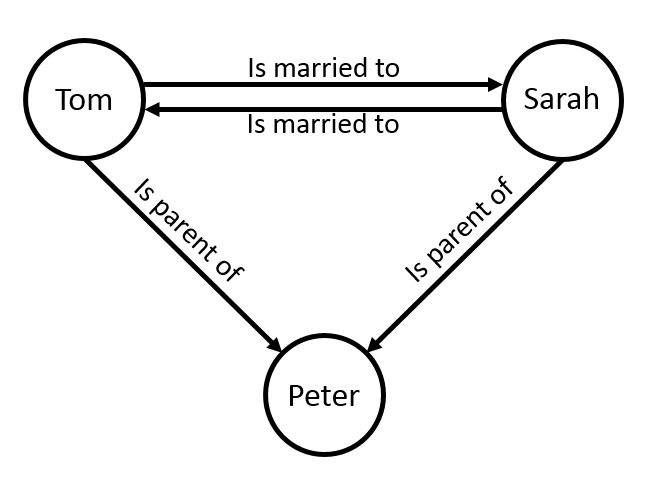
\includegraphics[width=.5\textwidth]{img/graph_example.PNG}
    \caption{A graph representing a small family. Tom, Sarah and Peter are entities and thus represented as nodes (circles). The two-way relationship between Tom and Sarah, their marriage, is depicted as two directed edges. Lastly, Tom and Sarah are the parents of Peter and thus both have the relationship "Is parent of" directed towards Peter.}
    \label{fig:graphdb:graph_example}
\end{figure}



\subsubsection{The property graph model}
The (labeled) property graph model is based on the theoretical graph from above \autocite{maheshlal2015}. It increases the overall information that a normal graph can store. Two such extensions, as the model name illustrates, are additional labels for each node and properties for nodes and edges. Figure \ref{fig:graphdb:property_graph_example} shows a labeled property graph.

\begin{figure}[ht]
    \centering
    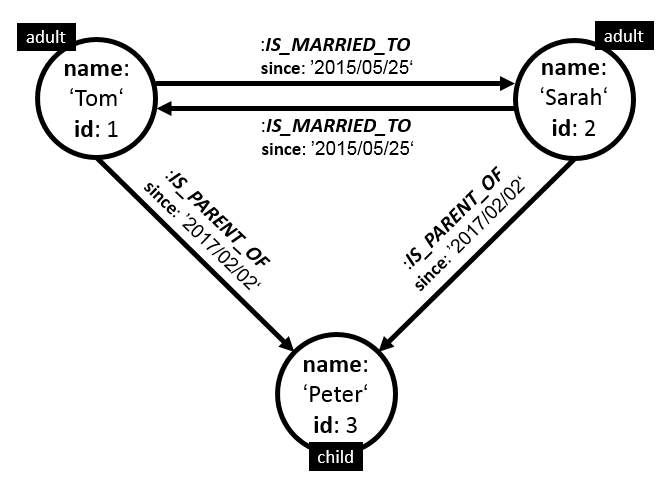
\includegraphics[width=.5\textwidth]{img/property_graph_example.PNG}
    \caption{A labeled property graph representing a small family \autocite{maheshlal2015, graphdb2015}. Compared to figure \ref{fig:graphdb:graph_example} additional information can been stored.}
    \label{fig:graphdb:property_graph_example}
\end{figure}

\scalebox{1}{\textbf{Concepts of the property graph}}

\textbf{Nodes:} Like a normal graph, the property graph represents entities as nodes. The nodes in figure \ref{fig:graphdb:property_graph_example} are the circles of Tom, Sarah and Peter. Each node can have any number of properties (e.g.: "name: ‘Tom’" and  "id: 1") and multiple labels (e.g. " adult") \autocite{neo4j:graphdb}.

\textbf{Labels:} Nodes are tagged with labels which describe the role of the node within the system \autocite{maheshlal2015}. In figure \ref{fig:graphdb:property_graph_example}, the white text on black rectangles, "adult" and "child", are labels. Labels can also add metadata (constraints and indices) to the node \autocite{maheshlal2015, neo4j:graphdb}.

\textbf{Properties:} Properties are attributes (key-value pairs) of nodes or relationships. They are used to sore further information about the entity or relationship \autocite{maheshlal2015}. Each bold and non-italic written word in figure \ref{fig:graphdb:property_graph_example} is a key of a key-value pair property (e.g. "name:", "id:", "since:"). The content that follows the colon (e.g. "Peter", "3", "2017/02/02") is the value.

\textbf{Relationships:} Again, relationship are depicted as directed edges (links) between nodes. Relationships must have a name as well as a start and end node \autocite{graphdb2015} . In figure \ref{fig:graphdb:property_graph_example}, \texttt{"IS\textunderscore PARENT\textunderscore OF"} and \texttt{"IS\textunderscore MARRIED\textunderscore TO"} (the italic and bold written words) are the names of relationships. The text below ("since: […]") is the property of the relationship. Arrows indicate the direction of the relationship.  In practice, the direction is ignored and navigation through each edge (relationship) is possible \autocite{maheshlal2015, neo4j:graphdb}. Generally, relationships store cost quantities according to the usage of the system (e.g. distance, ratings, etc.) \autocite{neo4j:graphdb}.

\subsubsection{Storage}
\blockquote{Storage deals with how the data is stored physically and how it is represented logically when retrieved}\autocite{maheshlal2015}

One of the main tasks of a graph database system is to traverse relationships. As mentioned earlier, storing and accessing the relationships in a graph database is crucial. They are stored explicit (per directed edge) instead of being inferred from stored attributes (like primary/foreign keys in a relational model) \autocite{maheshlal2015} . Thus, any kind of storage system needs to be able handle the relationships explicitly. Graph databases can either use native graph storage, systems that are built for storing and accessing graphs, or non-native graph storage, systems that store adequately transformed graph data in relational or non-graph NoSQL databases \autocite{graphdb2015}.

\scalebox{1}{\textbf{Non-native graph storage}}

Non-native graph storage transforms the data from the graph model (e.g. property graph) into relational or other non-graph NoSQL database models (document-oriented, etc.). When accessing the data, the responsible system must rebuild (infer) the relationships at runtime. This is mostly done by a query engine which is responsible for executing incoming queries and thus fetching or changing the data (CRUD methods) \autocite{maheshlal2015} . In the case of a relational database management system (RDBMS), the query engine would first make the relationships explicit by inferring them through utilizing foreign keys and join-statements before returning or processing the data. This preprocessing results in more costly operations and inefficient traversing of relationships \autocite{maheshlal2015}. Non-native graph storage exists because it allows the use of well known, mature and well documented databases like MySQL \autocite{graphdb2015}.

\scalebox{1}{\textbf{Native graph storage}}

The key aspect of native graph storage is that it does not rely on actual indexes. The relationships between nodes within the graph are “natural adjacency”\autocite{graphdb2015}  indices. Thus, the nodes are stored in such a way that they are physically linked to each other on the disk. This is called “index-free adjacency”\autocite{graphdb2015}, which is in practice done by pointers. Accordingly, searching for a specific information in a native graph storage is implemented by traversing through pointers. This causes queries on native storage to be highly efficient compared to non-native storage which uses join-statements and index lookups \autocite{graphdb2015} .

\subsection{Advantages of Graph Databases}
Graph databases offer substantial advantages when working with connected data \autocite{maheshlal2015}. Its performance, flexibility and agility are the key differences to other databases \autocite{graphdb2015}. The following section will take a closer look at these three advantages. More details and references to actual research data on these advantages can be found in the section Comparison: Graph Databases and Relational Databases (\ref{section:comparison}).

\subsubsection{Performance}
A graph database has much higher query processing performance compared to relational and other NoSQL databases. This advantage becomes more and more prevalent as the size/amount of stored data grows. In the relational world more data would mean a higher join-intensity and thus worse performance. Whereas in the graph database world the performance remains to be almost constant even for an exponential increase of size. This is the cases because queries are being restricted to parts of the graph (e.g. a subgraph) which contains the information of interest.  Therefore, querying only needs time proportional to size of the subgraph and not to the size of the whole graph \autocite{maheshlal2015, graphdb2015}.

\subsubsection{Flexibility}
The flexibility of a graph databases must be understood in the context of the graph database model. The model is flexible and so are graph databases. Furthermore, this flexibility is most apparent for an actual operational graph database in production environments.

The paradigm of fitting data to predefined data models, as in SQL, is neither efficient nor desired by developers. Instead fitting an easily extensible and changeable data model to newly emerging data is more appropriate for fields of graph database applications (See more in the section "Fields of Application”, \ref{section:FoA}). Thereby the process of designing a complex and mostly final data model at the start of the database implementation, a point in time where it is impossible to predict all kinds of data that might be needed in the future, gets replaced by designing a basic data model with the expectation to change it in the future \autocite{maheshlal2015, graphdb2015}.

This process is natively supported by graph databases. All components of a graph model (e.g. for the property graph model: nodes, properties, labels and relationships) can be added to an existing model without invalidating queries already in use. This concept of graph databases also minimizes maintenance cost and risk because the need for migrations (e.g. the equivalent of schema migrations for a relational database) is reduced \autocite{maheshlal2015, graphdb2015}.

\subsubsection{Agility}
In today's agile software development world, where developers need to focus on a certain task for a short time before switching to a different task, software tools that fit this iterative approach are more favorable. Databases that offer data models which can grow with new data meet this requirement. Additionally, databases that offer data models which do represent the data closer to its actual format (e.g. not transferring it into tables) are also more favorable because they reduce the time between design and implementation which is appropriate for the short time a developer may have to implement a database. Lastly, modern test-driven development requires agile databases to be easily testable. \autocite{maheshlal2015, graphdb2015}.

A graph database is “schema-less” \autocite{maheshlal2015}. It does not transform data (e.g. normalization in the SQL world) but rather tries to represent the data as close to its actual format as possible. Furthermore, the application programming interface (API) and query language design of graph database increase testability \autocite{graphdb2015} . Finally, the flexibility of its data model enables the database to evolve with new data. As a result, a graph database has the characteristics to be agile software.

\subsection{Fields of Application} \label{section:FoA}
When reading through use cases described by marketing teams of graph database management systems (for example: Neo4j \autocite{neo4j:why_graphdb, neo4j:use_cases}
), it may feel like any problem could be solved with a graph database. Solving any problem with a graph database may be possible but this fact alone is not a valid reason to do so.

Instead, cost efficiently, compliance with company polices, available developer skills and available time are the primary reasons to choose a graph database for a specific use case. Additionally, replacing existing well-working and established database management systems should have major and urgently needed advantages \autocite{graphdb2015}.

Graph databases can create these advantages for use cases which handle connected data. Below are some short examples of large companies that use graph databases. Subsequently, the top five use cases from the perspective of the graph database management system Neo4j are explained.

\subsubsection{Enterprise Use Case Examples}
\textbf{Social Networks:} Twitter, Facebook and LinkedIn use graph databases to manage user information and feed of users. This contains information like updates from friends, news and potential posts of relevance or interest (e.g. Jobs for LinkedIn users) \autocite{maheshlal2015}.

\textbf{Routing:} Prominent navigation services like Google Maps, TomTom and Sygic utilize graph databases for map navigation \autocite{maheshlal2015}.

\textbf{Search:} Google (Google Knowledge Graph) and Facebook (Facebook Social Graph) are also using graph databases for storing the connection of content for search functionalities \autocite{maheshlal2015}.

\textbf{Recommendation:} Walmart and eBay are both using graph databases and value their performance for real-time product recommendations \autocite{neo4j:use_cases}.

\subsubsection{Neo4j Use Cases}
\scalebox{1}{\textbf{Fraud Detection}}

Graph databases are well fit for fraud detection because good detection mechanisms need to analyze the relationships between data. In detail, if the relationships between certain data objects is conspicuously high, the risk of fraud is very high.  As an example, take an E-commerce system. A normal user would use one or two credit cards to buy products. A fraudster would use a lot of different credit cards which are most likely stolen. This relationship density between users, credit cards and purchased products is modeled by a graph database and is therefore easily measurable and observable \autocite{neo4j:use_cases}.

As mentioned before, graph databases are built for storing and rapidly traversing relationships, thereby supporting advanced detection mechanisms that need to perform relationship analysis between a lot of data.

\scalebox{1}{\textbf{Real-Time Recommendation Engines}}

A real-time recommendation engine can only be as effective as the database it is using because the engine needs information about the existence, quality and strength of data relationships. Information must either be computed from the database in a time-consuming manner or made available natively, as with graph databases \autocite{neo4j:use_cases}. Graph databases model this information without any additional computation. Existence is modeled by edges (relationships), quality and strength by key-value pairs (properties) of edges.

In addition, the need to easily add and combine data (e.g. user behavior, demographics and their purchase history) and then analyze this new dataset in real time for possible recommendations is crucial for such an engine \autocite{neo4j:use_cases}. A graph database supports simple addition and combination with its already mentioned flexibility. Furthermore, the performance advantage of graph databases in this context is again very favorable when analyzing this new dataset.

\scalebox{1}{\textbf{Master Data Management}}

In a company, master data is data such as users, customers, products, accounts, partners, sites and business units. Identifying, cleaning, storing and governing this data is called Master data management (MDM). Best practice for MDM is to create one master data store which contains the data of the entire company. As a result, any business application that might create or use this data only uses only the same storage system. Hence, the master data store is one storage system for a lot of different applications which still needs to fully function in real time and might need to adapt to new business requirements. Thus, it must provide a purpose-built, dynamic and sometimes unconventional data model \autocite{neo4j:use_cases}. These requirements are perfectly matched by the flexibility and agility of a graph database.

\scalebox{1}{\textbf{Network and Information Technology Operations}}

The structural representation of an information technology (IT) infrastructure network is a graph. Consequently, it should not be a surprise that a graph database is a good solution to model, store and serve requests for an IT infrastructure environment. Information in an IT infrastructure environment are for example device configurations, infrastructure interdependencies, any kind of event (log files, error messages, etc.) and administrative details. Systems that use such information can, in the event of a failure, inform the right administrator about what went wrong where and when in real time \autocite{neo4j:use_cases}.

A graph database is not only able to model the network in its native representation but is also able to add all this information to its storage with ease. Network administrators are nodes with connection to their devices and field of responsibility (subgraphs). Configurations are properties of device nodes. Any interdependencies are represented by relationships. Lastly, events are nodes linked to the device that created it. This requirement for a native data model and sufficient performance is fulfilled by a graph database.

\scalebox{1}{\textbf{Identity and Access Management}}

The process of deciding which identity can access which resource is called identity and access management (IAM). This decision process also needs to utilize information about identities (e.g.  administrators, users), resources (e.g.  files, devices) and rules (e.g. “user X can access file Y”) that must be stored somewhere. Conventional storage options, like directory services or application specific solutions, tend to be unsuitable because they cannot manage the required complex interconnection structures of big organizations or are too slow for bigger datasets \autocite{neo4j:use_cases}.  Whereas a graph database is a valid solution because its agility allows the developer to easily model the complex structures and its performance does not slow down for bigger datasets.


\subsection{Comparison: Graph Databases and Relational Databases} \label{section:comparison}
The comparison between Graph Databases and Relational Databases is a known field, a lot of literature exists on this topic already. Throughout the comparisons, the two methods are always assessed under the same aspects: performance, flexibility, security and maturity. \\
For those comparison points it makes sense to focus on specific implementations of the technologies, hence in this section Neo4j will be chosen as a concrete precedent for Graph Databases, whereas MySQL will be the example implementation for Relational Databases. \\
It is important to note that literature comparing the two is already rather old and there are no comparisons done on newer versions. There is no new version of mySQL, but two new releases for Neo4j. Those have included a new query engine and performance optimizations. It is hence expected that if such a comparison were to be done again today, the performance results of Neo4j would improve.

\subsubsection{Performance} \label{sec:graphdb:performance}
Detailed surveys on performance of both technologies already exist in literature, for example from Vicknair et al. \autocite{Vicknair2010}. In this specific instance, MySQL version 5.1.42 and Neo4j-b11 were compared.
The queries chosen for the experiments were similar to types that are used in real world provenance systems. Typically in this scenario, for one node one traverses the graph to find its origin. Another use case in this context is, if a data object or node is deemed incorrect, this information needs to be propagated to all its descendants/child nodes \autocite{Vicknair2010}.\\
Further on, the queries were partitioned into structural queries referencing the graph but not the payload itself, and data queries using the actual payload data. It is important to note that the payload data in this case was integer payload data, as different types are handled separately depending on the framework.\\
In the traversal queries, Neo4j clearly outperformed MySQL, sometimes even being faster by the factor of 10. Though that was expected, as Relational Databases are not designed for traversals. MySQL for this part of experiment falls back to a standard Breadth First Search, which is not optimal for this scenario. Neo4j on the other hand has a built in framework for traversals, making it superior in terms of performance for the traversal queries \autocite{Vicknair2010}. \\
Contrary to that, in the data queries MySQL turned out to be more efficient. This result was partly due to the fact that Neo4j uses Lucene for querying, which treats all payload as text, even though in this scenario the payload is of type integer. But also when the payload changes to text, MySQL had better performance in the experiments \autocite{Vicknair2010}. Lucene has since been dropped and replaced with Cypher in Neo4j version 3.\\
The researchers also took into account a special case for the experiments, trying the data queries with payload that is closer to actual real world data - text with spaces in between the words. Surprisingly, at a large enough scale Nao4j outperformed MySQL by a large amount for those queries.

\subsubsection{Flexibility}
The flexibility aspect compares both database technologies in their behaviour when taken out of the environment that they were created for \autocite{Vicknair2010}. \\
For Relational Databases an uncommon environment would for example be ad-hoc data schemes that change with time, whereas for Graph Databases a less typical dataset would be one without many connections between the individual nodes  \autocite{GarimaAnalysis}.
MySQL is optimized for a large-scale multi-user environment, hence trying to use it for smaller applications comes with a large overhead of functionality that has to be implemented with it but that may not even be needed for this specific application.
Neo4j is typically targeted towards more lightweight applications, but manages to scale really well, having a scalable architecture that also accounts for speed \autocite{neo4jweb}. Its easily mutable schema makes it more flexible with data types that are rather untypical for Graph Databases.

\subsubsection{Security}
Neo4j does not have built in mechanisms for managing security restrictions and multiple users in their community edition \autocite{GarimaAnalysis}, but the fee-based enterprise edition provides such functionality. MySQL on the other hand natively supports multiple users as well as access control lists. \autocite{mysqlsecurity}

\subsubsection{Maturity}
For the comparison under the aspect of maturity it makes sense to talk about database implementations in general. Maturity refers both to how old a particular system is and to how thoroughly tested it is \autocite{Vicknair2010}.
Since all Relational databases - including MySQL - use the same query language SQL, support is equal over all implementations and support for one implementation is applicable to all others \autocite{GarimaAnalysis}.
Neo4js version 1.1 was released in February 2010. While Neo4j is a for-profit framework and has decent support from its parent company, this does not apply to all graph database implementations \autocite{Vicknair2010}. Furthermore, the query languages differ from implementation to implementation, separating them in that aspect and making support for one implementation not applicable to another one.

\section{Implementing a Graph Database Model} \label{section3}
This section shall outline the general approach, how to convert an existing relational database model into a property graph model.
In the second part an introduction to Neo4j, the implementation of a database model in Python and basic querying in an application and with Neo4js own query language \glqq Cypher\grqq{} will follow.

\subsection{Converting a Relational Database Model}
There are a couple of guides available describing how to build a database model for Neo4j. Since the database itself is schema-less, multiple schemas can be used and implemented at the same time.
Nevertheless an application needs a model of the data.
Neo4j states in \autocite{neo4j:rel_to_graph} that it is possible to transfer almost all existing relational models into a graph model.
The general approach has been described in \autocite{dzone:rel_to_graph}.
The first step in this conversion is to consider the names of all Non-JOIN-Tables as labels.
Foreign keys will become relations.
JOIN-Tables will be converted into relations as well with additional properties added to the relation \autocite{neo4j:graph_vs_rdbms}.
The rows will be converted into nodes connected by edges based on the formerly converted relations. Attributes not covered in the previous steps will become properties of a node.

\subsection{Implementing a sample project with Neo4j}
In this section the modeling and setup with Neo4j will be lined out and a sample project be described utilizing available Python-Libraries to implement a sample project.
There are two different available versions of Neo4j.
First of all there is the Open Source community edition which is published under the GPL.
Additionally Neo4j Inc sells licenses for an enterprise edition \autocite{neo4j:editions} including support and several additional features, such as replication, multiple users, several query performance optimizations and no limitation for the number of nodes in the database (the community version is limited at 34 Billion nodes).
The following examples have been implemented and tested with the community edition.

\subsubsection{Setting up Neo4j}
Neo4j is available for Windows, Linux and Mac and can be installed via the provided packages. While there is a minimum requirement of 2GB of RAM, Neo4j recommends 16GB or more \autocite[Chapter~2.1]{neo4j:op_manual}.
Since Neo4j is implemented in Java, starting it can be done by invoking it with a Java runtime of choice installed. The default configuration does not need to be modified to get started.

\paragraph{High availability} \label{par:graphdb:ha} The community edition of Neo4j does not allow to set up a cluster of multiple Neo4j instances.
This feature is reserved for the enterprise version.
The setup of a causally consistent cluster is explained in the documentation \autocite[Chapter~5.1]{neo4j:op_manual}.
The reference architecture as shown in \autoref{fig:graphdb:causal_cluster} recommends an odd number of at least three \glqq Core Servers\grqq{} connected into a RAFT-Cluster handling mostly write requests.
They ensure consistency of the data.
Connected to this core cluster may be an arbitrary number of \glqq Read Servers\grqq.
They only handle the -- sometimes resource costly -- read requests but are not relevant to the clusters integrity.
Information from Core Servers is replicated asynchronously to the read replicas.
\begin{figure}[ht]
    \centering
    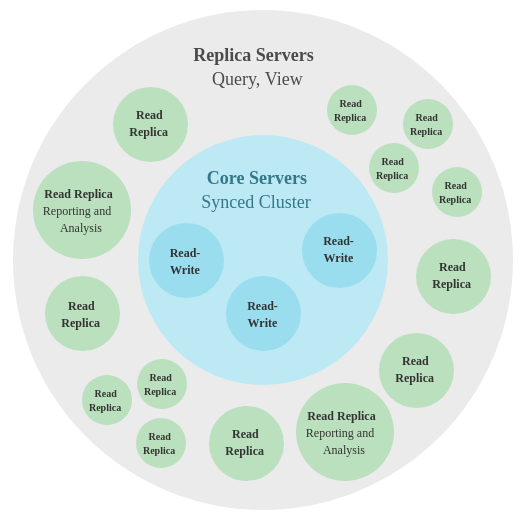
\includegraphics[width=.5\textwidth]{img/causal_clustering.png}
    \caption{Neo4j causal Cluster Architecture \autocite[Chapter~5.1]{neo4j:op_manual}}
    \label{fig:graphdb:causal_cluster}
\end{figure}

\paragraph{Classification of Neo4j within the CAP Theorem} For this kind of classification it is again necessary to differentiate between the community and the enterprise edition.
Since it is not possible to set up a Neo4j-Cluster with the community edition it can not be considered a distributed system.
Therefore the CAP-Theorem is not applicable \autocite{dzone:understanding_cap}.

As mentioned in \autoref{par:graphdb:ha} the enterprise edition can be set up as a causal cluster.
Causal consistency though does not fulfill the criteria Brewer put out for consistency \autocite{DBLP:journals/corr/Kleppmann15} so it can not be considered as \glqq C\grqq{} under the CAP Theorem.
It is important to note that a causal cluster is still ACID compliant.
Due to the nature of the core servers using a consensus-based protocol (RAFT) availability in case of a network partition only applies to the majority of the cluster \autocite{infoq:neo4j}.
This does make them partition tolerant though, fulfilling all criteria for \glqq P\grqq.

According to Michael Hunger, one of the Neo4j developers, the causal cluster architecture can be considered as a \glqq CP\grqq{} system \autocite{infoq:neo4j}.
Considering the the concerns lined out by Martin Kleppmann in his blog post \autocite{kleppmann:caprant} Neo4j should be considered as \glqq P\grqq{} -- if no alternative to CAP is considered as proposed by him \autocite{DBLP:journals/corr/Kleppmann15}.


\subsubsection{Modeling the graph database}
The sample project maps the relations within users in a social network.
\autoref{fig:graphdb:graphmodel} outlines a data model with circles representing nodes. They are connected by edges showing their relationships.
For this example labels are represented as colours.
In this sample model there may be an arbitrary number of persons (orange), who may be friends with other persons.
Additionally, they can share interests (green) and may be a member of a group (purple).
Furthermore they can state from which country (yellow) they are from.

\begin{figure}[H]
    \centering
    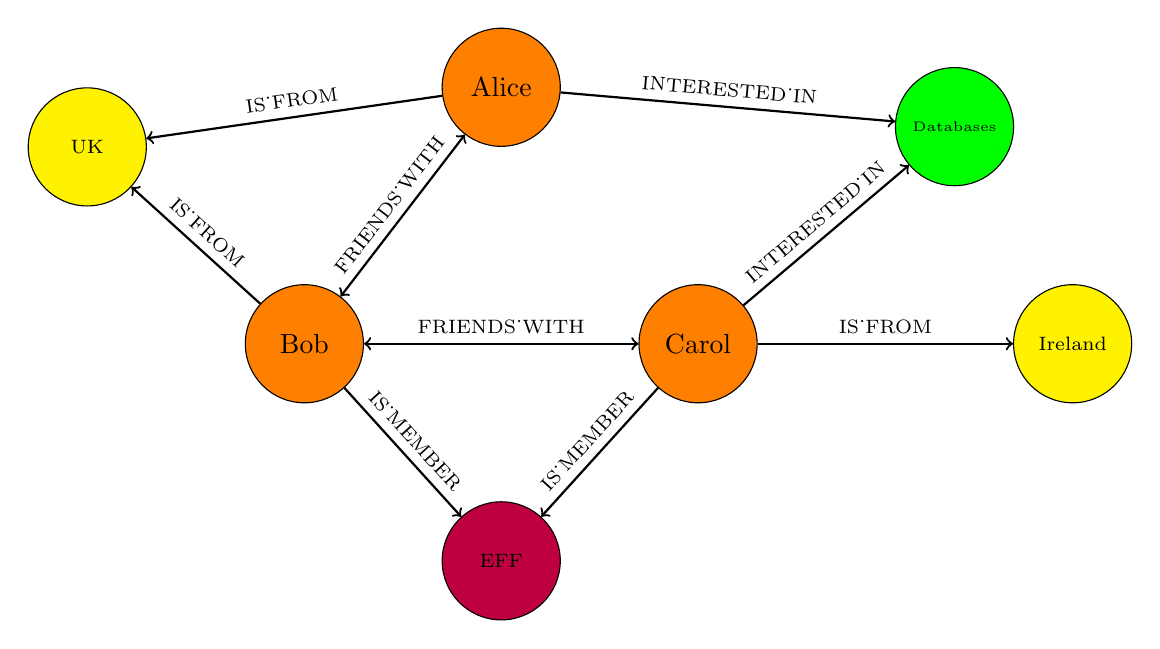
\begin{tikzpicture}
        \node[draw, circle, fill=orange, minimum height=1.5cm, minimum width=1.5cm] (alice) {Alice};
        \node[draw, circle, fill=orange, minimum height=1.5cm, minimum width=1.5cm] (bob)  at ([xshift=-2.5cm, yshift=-2.5cm]alice.south) {Bob};
        \node[draw, circle, fill=orange, minimum height=1.5cm, minimum width=1.5cm] (carol)  at ([xshift=2.5cm, yshift=-2.5cm]alice.south) {Carol};

        \node[draw, circle, fill=green, minimum height=1.5cm, minimum width=1.5cm] (db) at ([xshift=5cm, yshift=-0.5cm]alice.east) {\tiny Databases};

        \node[draw, circle, fill=purple, minimum height=1.5cm, minimum width=1.5cm, align=center] (eff) at ([xshift=2.5cm, yshift=-2cm]bob.south) {\scriptsize EFF};

        \node[draw, circle, fill=yellow, minimum height=1.5cm, minimum width=1.5cm] (uk) at ([xshift=-2cm, yshift=2.5cm]bob.west) {\scriptsize UK};
        \node[draw, circle, fill=yellow, minimum height=1.5cm, minimum width=1.5cm] (ire) at ([xshift=4cm]carol.east) {\scriptsize Ireland};



        \draw [<->, thick] (alice) -- (bob) node[midway,sloped, above] {{\scriptsize FRIENDS\char`_WITH}};

        \draw [<->, thick] (bob) -- (carol) node[midway,sloped, above] {\scriptsize FRIENDS\char`_WITH};

        \draw [->, thick] (alice) -- (db) node[midway,sloped, above] {\scriptsize INTERESTED\char`_IN};
        \draw [->, thick] (carol) -- (db) node[midway,sloped, above] {\scriptsize INTERESTED\char`_IN};

        \draw [->, thick] (bob) -- (eff) node[midway,sloped, above] {\scriptsize IS\char`_MEMBER};
        \draw [->, thick] (carol) -- (eff) node[midway,sloped, above] {\scriptsize IS\char`_MEMBER};

        \draw [->, thick] (alice) -- (uk) node[midway,sloped, above] {{\scriptsize IS\char`_FROM}};
        \draw [->, thick] (carol) -- (ire) node[midway,sloped, above] {{\scriptsize IS\char`_FROM}};
        \draw [->, thick] (bob) -- (uk) node[midway,sloped, above] {{\scriptsize IS\char`_FROM}};

    \end{tikzpicture}
    \caption{Sample database schema}
    \label{fig:graphdb:graphmodel}
\end{figure}

\subsubsection{Implementation in Python}
While it is possible to manage the database utilizing the CRUD-functionality from Neo4js own query language Cypher (see \ref{sec:graphdb:cypher}) this is not really suitable for an application.
Developers familiar with Object-Relational-Mappers (ORM) such as Hibernate for Java or SQLAlchemy for Python would prefer to define the different nodes and relations in classes providing the database elements as objects and abstracting actual SQL-Queries.

For Python there exists a community driven project called neomodel \autocite{github:neomodel} aiming to provide an Object-Graph-Mapper (OGM) for Python projects. Neomodel is published under the MIT License.

\begin{listing}[ht]
    \begin{minted}{python}
    class Partnership(StructuredRel):
        since = DateTimeProperty(
            default=lambda: datetime.now(pytz.utc)
        )

    class Country(StructuredNode):
        name = StringProperty(unique_index=True, required=True)

    class Interest(StructuredNode):
        name = StringProperty(unique_index=True, required=True)

    class Group(StructuredNode):
        name = StringProperty(unique_index=True, required=True)

    class Person(StructuredNode):
        uid = UniqueIdProperty()
        name = StringProperty(unique_index=True)
        age = IntegerProperty(index=True, default=0)

        # traverse outgoing relations
        country = RelationshipTo(Country, 'IS_FROM')
        interests = RelationshipTo(Interest, 'IS_INTERESTED_IN')
        groups = RelationshipTo('Group', 'IS_MEMBER')
        friends = Relationship('Person', 'FRIENDS_WITH', model=Partnership)
    \end{minted}
    \caption{Example graph database model with neomodel}
    \label{lst:graphdb:neomodel}
\end{listing}

The implementation of the graph model mentioned in \autoref{fig:graphdb:graphmodel} in Python has been realized in \autoref{lst:graphdb:neomodel} following the neomodel documentation \autocite{neomodel:rtd}. With this model it is possible to create new nodes in the database by instantiating a new object of the given classes as in \autoref{lst:graphdb:createPerson}.
\begin{listing}[H]
\begin{minted}{python}
lmeitner = Person(name='Lise Meitner', age=89)
lmeitner.save()
\end{minted}
\caption{Creating a new person node in the database}
\label{lst:graphdb:createPerson}
\end{listing}

To connect two nodes it is necessary to get both objects and to invoke the \texttt{connect()} method as seen in \autoref{lst:graphdb:connectNodes} on one of them.
The \texttt{get\char`_or\char`_create} method simplifies creation of nodes with no additional properties since it either returns an already existing node or creates it.
\begin{listing}[H]
\begin{minted}{python}
country = Country.get_or_create({'name': 'Austria'})
lmeitner.country.connect(country[0])
\end{minted}
\caption{Connecting a person and a country node}
\label{lst:graphdb:connectNodes}
\end{listing}

Retrieving one or more existing nodes can be done by filtering as shown in \autoref{lst:graphdb:queryPerson}.
\begin{listing}[H]
\begin{minted}{python}
curie = Person.nodes.filter(name='Marie Curie')
\end{minted}
\caption{Querying for a person node by the name attribute}
\label{lst:graphdb:queryPerson}
\end{listing}

\subsubsection{Queries using Cypher}
\label{sec:graphdb:cypher}
Neo4j provides its own query language Cypher. It is developed with an open source specification called openCypher \autocite{openCypher}.
Thus it should be possible to use the same query language for graph processing in other databases -- such as SAP HANA or Redis.
Its syntax is oriented on SQL statements though there are quite some differences to better match with a graph model.
Neo4j has an extensive introduction how to use Cypher \autocite{neo4j:cypher_introduction}.
Therefore only a short introduction should be given here.

Cypher uses two basic patterns.
First of all there are nodes, denoted by enclosing parentheses.
The second pattern is used for relationships.
They are expressed by two dashes and may have a direction utilizing the greater-than/less-than signs.
Furthermore, the type of a relationship may be specified in brackets between the two dashes.

A few examples will make it easier to understand how these patterns can be used.

The simplest query would be to get all nodes and all relations between them without regard to their labels.
This can be achieved by calling \mint{SQL}|MATCH (n) RETURN n|
It is important to note that Cypher uses \texttt{MATCH} as a keyword similar to SQLs \texttt{SELECT}.
Contrary to SQL it is necessary in Cypher to \texttt{RETURN} the previously matched nodes to obtain them in the result.
It is possible to declare the label of a node by calling \mint{SQL}|MATCH (p:Person) RETURN p|
This would reduce the output to all persons and the relations between them.

As mentioned before Cypher supports a pattern for relations.
To include them in a query -- e.g. for all Persons who have one or more friends the query would look like \mint{SQL}|MATCH (a:Person) -[:FRIENDS_WITH]- (b:Person) RETURN a, b|
The relationship type in the brackets may be ommited to get all types of relations between these nodes.

Similar to SQL, Cypher also supports a \texttt{WHERE} statement.
To query for a specific Person where the attribute \texttt{name} equals \glqq Otto Hahn\grqq{} and all nodes connected to this person the Cypher query would look like this \mint{SQL}|MATCH (p:Person)-[r]-(n) WHERE p.name = 'Otto Hahn' RETURN p, r, n|

Of course Cypher offers a complete keyword set for all types of CRUD operations. Interested readers should follow the introduction by Neo4j \autocite{neo4j:cypher_introduction}.

\subsection{Conclusion}
Getting started with Neo4j is relatively simple.
There is plenty of documentation available helping to implement a database model and an application based on it.
Especially the OGM Projects for Python are pretty advanced and suitable for production usage.
Users familiar with SQL will find Cypher not that difficult to get used to.

There are two major downsides to Neo4j. The first one is the memory footprint.
A newly set up instance already consumes more than 600MB of RAM -- in comparison, a PostgreSQL instance storing a couple hundred MB of data still consumes less than half of that.
The second downside is, that many features -- especially regarding maintenance and clustering -- are preserved for the enterprise edition and not available in the open source community edition. This makes it difficult if not impossible to use the community edition in a production environment.

\section{Reflection} \label{section4}
\subsection{Alternative popular Graph Databases}
\subsubsection{OrientDB}
OrientDB is one of the biggest competitors to Neo4j, developed by Callidus Software Inc. (owned by SAP) and published under Apache-2 License \autocite{orientdb:vs_neo4j}.
Like Neo4j it is implemented in Java.
OrientDB is a multi model graph database, just as Neo4j, but also a document oriented database allowing relations between documents \autocite{orientdb:why}.
As a query language OrientDB uses SQL with a custom dialect to include features for traversals \autocite{orientdb:vs_neo4j}.
In comparison to Neo4j they claim to be a lot faster \autocite{orientdb:vs_neo4j}.
This claim is based on a paper \autocite{cloudcom:2012}, which has been released in 2012.
As mentioned in \autoref{sec:graphdb:performance} Neo4j has reimplemented their query engine since then.


A major selling point is the possibility to set up a highly-available (multi-master) cluster of multiple nodes with the Open Source community version \autocite{orientdb:cluster, orientdb:support}.

\subsection{Conclusion}
Even though there is extensive literature on the topic of Graph Databases, our group was overall dissatisfied with the scientific resources we found. Most publications were written by the same few people, not providing a distinct enough reflection on the topic. Furthermore, while there were many publications around 2010 on this topic, literature did not provide updates or added benchmarks of e.g. comparisons with other database systems. We aim to close that gap with an updated summary on today's Graph Database theory and Neo4j. \\
In this chapter, we first gave an introduction into Graph Databases, providing an overview of its history. Next, the basic underlying theory was explained and assessed critically. A report on the implementation with Neo4j was given, stating its distinct characteristics and concluding its value as a Graph Database implementation.

To conclude, we would also like to share our personal experience of working with Neo4j and Graph Databases in general. Overall, we feel that with the concept of Graphs as a database model one can easier map real life datastructures than with just a relational structure. While the underlying theory is rather complex, we felt that there were sufficient resources to give a simple introduction into the topic. The implementation was enjoyable, as the documentation for Neo4j was easily understandable and it did not take long until the basic setup was complete. We especially enjoyed using community driven libraries; when issues arose we were given an answer and help immediately, making our experience overall very pleasant.

Future work to extend this paper could include assessing the enterprise edition. We were unable to compare the community edition to the enterprise edition due to stellar pricing. The fee-based version allows for clustering which would have been interesting to take into account for our implementation. In addition, a deeper evaluation of alternatives like OrientDB could be valuable, especially since OrientDB is an open source project and provides clustering functionality in its community version. Lastly, Hypergraph and Triplet propose interesting approaches to graph modeling and an assessment of the differences and strengths would be valuable for the current literature landscape.
